\section{Initial Control Design}
%
It is desired to design a state feedback using a linear quadratic regulator (LQR). As the controller eventually must be implemented the design is carried out in the discrete domain. To do so, it is necessary to discretize the system. A discrete state space model can be expressed as,
%
\begin{flalign}
  \vec{x}(k+1) &= \vec{A_z} \vec{x}(k) + \vec{B_z} \vec{u}(k)
  \label{xDotLinearDiscrete} \\
  \vec{y}(k)   &= \vec{C_z} \vec{x}(k) + \vec{D_z} \vec{u}(k) \ \ ,
  \label{yLinearDiscrete} 
\end{flalign}
%
where the z subindexes indicate the matrices being in the discrete domain and k is the sample index. The model is discretized using zero order hold. In \autoref{fig:discreteSSBlock} the discrete system is shown in a block diagram. The feed forward matrix is excluded as it is not present in this system.
%
\begin{figure}[H]
  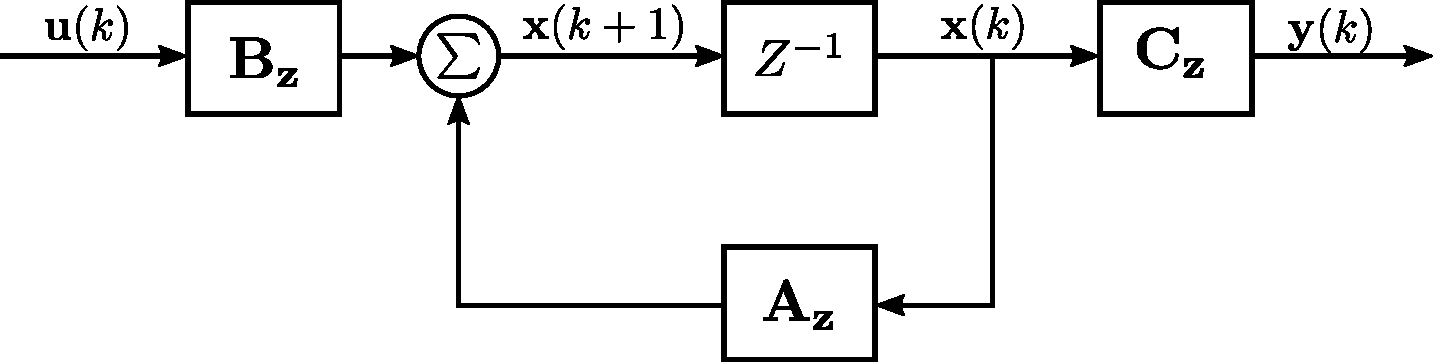
\includegraphics[width=0.6\textwidth]{figures/discreteSystemBlockDiagram}
  \caption{Block diagram of the discrete system without feed forward.}
  \label{fig:discreteSSBlock}
\end{figure}
%
\fxnote{talk about controllability here.}
%
In order to track a reference and handle input disturbances, it is chosen to also include an integral controller in the design. The final control structure is seen in \autoref{fig:blockConrolDesignLQR}.
%
\begin{figure}[H]
  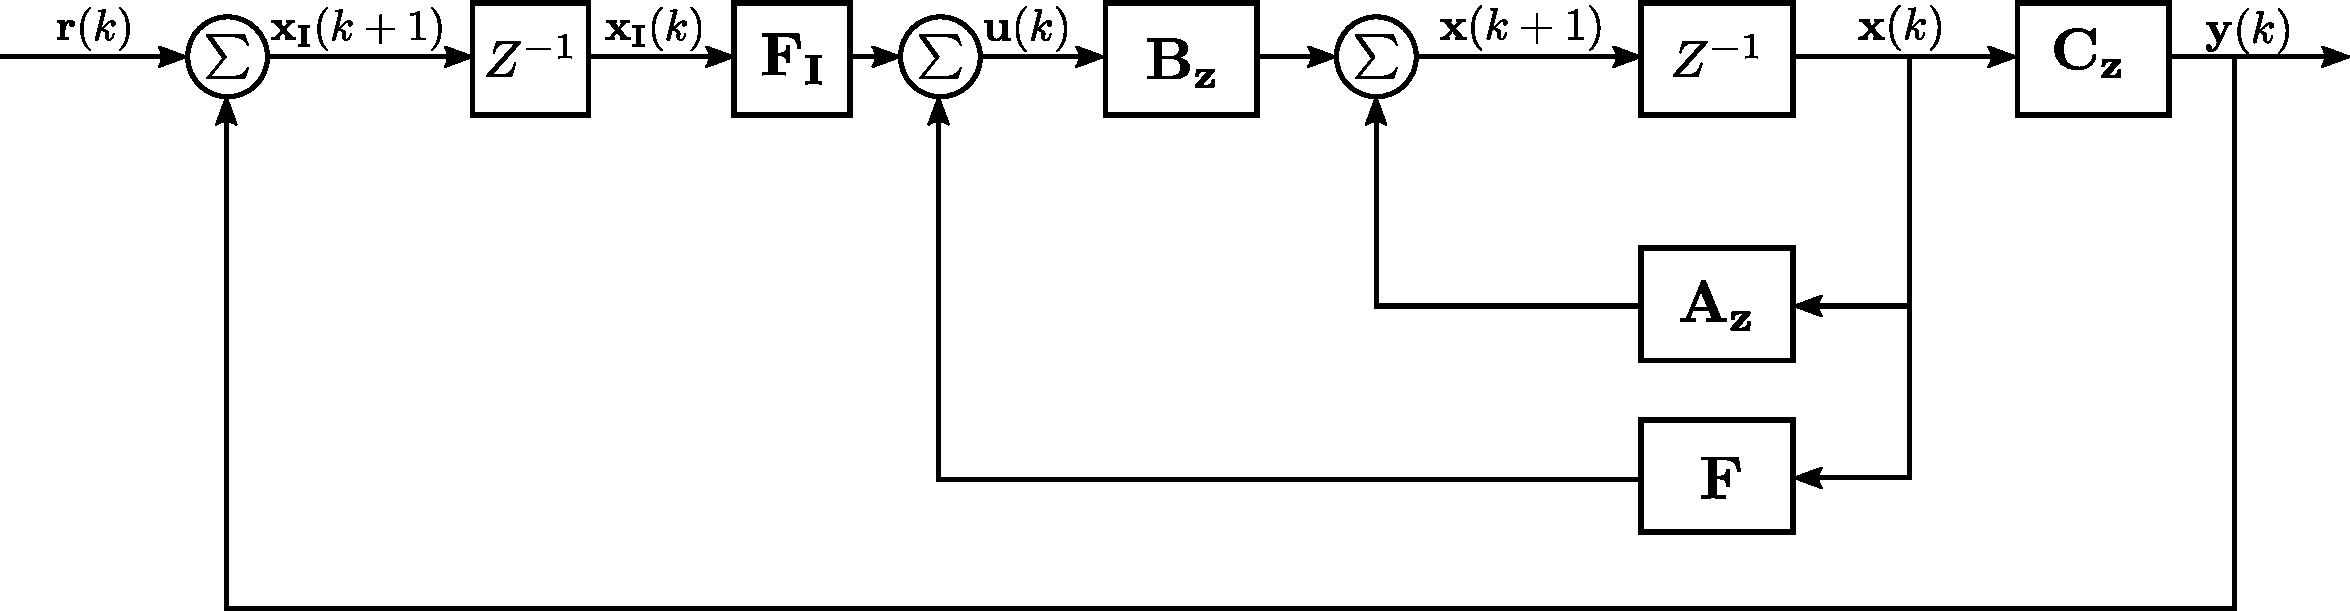
\includegraphics[width=0.9\textwidth]{figures/integralControlBlockDiagram}
  \caption{Block diagram of the control structure in the discrete domain.}
  \label{fig:blockConrolDesignLQR}
\end{figure}
%
To design this feedback system, it is convenient to express it on the following form:
\begin{flalign}
  \vec{x_e}(k+1) &= \vec{A_e} \vec{x}(k) + \vec{B_e} \vec{u}(k) + \vec{r}(k)
  \label{eq:xDotLinearDiscrete} \\
  \vec{y}(k)     &= \vec{C_e} \vec{x}(k)  \ \ .
  \label{eq:yLinearDiscrete} 
\end{flalign}
%
To describe the control design in this form, the $\vec{A_e}$, $\vec{B_e}$ and $\vec{C_e}$ matrices must be constructed. From \autoref{fig:blockConrolDesignLQR}, following relation is found:
%
\begin{flalign}
  \vec{x_I}(k+1) &= \vec{x_I}(k) + \vec{y}(k) + \vec{r}(k)    \nonumber \\
  \vec{x_I}(k+1) &= \vec{x_I}(k) - C_z \vec{x}(k) + \vec{r}(k)  \ \ .
  \label{eq:xIDiscrete}
\end{flalign}
%
This leads to the discrete state space model extended with the integral state expressed as
%
\begin{flalign}
  \begin{bmatrix}
    \vec{x}(k+1)  \\
    \vec{x_I}(k+1)
  \end{bmatrix}
  =
  \begin{bmatrix}
    \vec{A}_{\vec{z}_{3x3}} & \vec{O}_{_{3x2}} \\
   -\vec{C}_{\vec{z}_{2x3}} & \vec{I}_{_{2x2}} \\
  \end{bmatrix}
  \begin{bmatrix}
    \vec{x}(k)    \\
    \vec{x_I}(k)
  \end{bmatrix}
  +
  \begin{bmatrix}
    \vec{B}_{\vec{z}_{3x2}} \\
    \vec{O}_{2x2}
  \end{bmatrix}
  \vec{u}(k)
  +
  \begin{bmatrix}
    \vec{O}_{3x2} \\
    \vec{I}_{2x2}
  \end{bmatrix}
  \vec{r}(k)
  \label{eq:discreteSSWithIntegralX}
\end{flalign}  
%
\begin{flalign}
  \vec{y}(k)
  =
  \begin{bmatrix}
    \vec{C}_{\vec{z}_{2x3}} &  \vec{O}_{2x2}
  \end{bmatrix}
  \begin{bmatrix}
    \vec{x}(k)    \\
    \vec{x_I}(k)
  \end{bmatrix}  \ \ ,
  \label{eq:discreteSSWithIntegralY}
\end{flalign}  
%
which cooresponds to \autoref{eq:xDotLinearDiscrete} and \ref{eq:yLinearDiscrete}.

A discrete time infinite horizon LQR is used in the design of the feedback, $\vec{F_e} = [\ \vec{F} \ \ \vec{F}_\mathrm{I} ]\ $, which works by minimizing the cost function,
%
\begin{flalign}
  J = \sum_{k=0}^\infty \vec{x}_k^\mathrm{T}\vec{Q}\vec{x}_k + \vec{u}_k^\mathrm{T}\vec{R}\vec{u}_k \ dt \ \ .
\end{flalign}
\begin{where}
	\va{\vec{Q}}{is the state cost matrix}{}
  \va{\vec{R}}{is the input cost matrix}{}
\end{where}

The Q matrix contains the penalties for the state, such that a higher cost is generated for more critical states, thus driving these states faster to zero. The R matrix contains the penalties for the input. This helps to ensure that the actuators never enters saturation.
Bryson's rule is used to determine sensible values for the state and input penalties in the Q and R matrices.
%
\begin{flalign} 
Q_{ii} &= \frac{1}{[x_{i_\mathrm{max}}]^2} \ \ \ \ R_{ii} = \frac{1}{[u_{i_\mathrm{max}}]^2}
\label{eq:QRBryson}
\end{flalign}
\begin{where}
  \va{x_{i_\mathrm{max}}}{are the maximum acceptable state values}{}
  \va{u_{i_\mathrm{max}}}{are the maximum acceptable input values}{}
\end{where}

From this the state feedback is calculated by,
%
\begin{flalign} 
  \vec{F}_\mathrm{e} &= (\vec{R} \vec{B}_\mathrm{e}^\mathrm{T} \vec{P}\vec{B}_\mathrm{e})^{-1}  \vec{B}_\mathrm{e}^\mathrm{T} \vec{P}\vec{B}_\mathrm{e}
  \label{eq:QRFeedback}
\end{flalign}
\begin{where}
  \va{\vec{P}}{is the state transfer matrix.}{}
\end{where}

$\vec{P}$ provides a feedback matrix which minimizes the cost function, and can be found by use of the Riccatti equation.
%$\vec{F}_\mathrm{e}$ can be seperated to make F and F_I as the first 6 columns are state feedback and the last three are the integral control. These feedback matricees can can be implemented as shown in \autoref{fig:blockConrolDesignLQR}.











